\documentclass[11pt, a4paper]{article}

% -- Packages ------------------------------------------------------------------
\usepackage[utf8]{inputenc}
\usepackage[T1]{fontenc}
\usepackage[english]{babel}
\usepackage{lmodern}
\usepackage[margin=2.5cm]{geometry}
\usepackage{amsmath, amssymb, amsthm}
\usepackage{graphicx}
\usepackage{tikz}
\usepackage{xcolor}
\usepackage{microtype}
\usepackage{parskip}
\usepackage[above,below]{placeins}
\usepackage{hyperref}

\hypersetup{colorlinks=true, linkcolor=black, citecolor=teal, urlcolor=teal}

\newcommand{\R}{\mathbb{R}}
\newcommand{\vOS}{\textsf{vOS}}
\newcommand{\nucleus}{\texttt{vsf-nucleus}}

% -- Title  --------------------------------------------------------------------
\title{%
  \textbf{Convergence to a Geometric Attractor in a Viable System Kernel}\\[4pt]
  \large Executive Summary --- June 2026
}

\author{Luis Pineda R.\\
  \small Independent researcher --- Valpara\'{i}so, Chile\\
  \small \href{mailto:luis@tallerpineda.cl}{\texttt{luis@tallerpineda.cl}}}
\date{\textit{Technical Report --- April 2026; revised June 2026}}

\begin{document}
\maketitle

% ==============================================================================
\section*{What We Built}

We constructed a computational kernel (\nucleus{}) based on Beer's Viable System
Model (VSM) and tested whether a system governed by a minimal set of cybernetic axioms
converges to a stable attractor in state space. The kernel's state is a point in
$\R^{128}$, organised into semantic blocks: identity, resources, entropy, operations,
communication channels, attractor memory, and regulatory intelligence.

We ran over thirty-five experiments on physical hardware (Intel Core i7-7600U, Proxmox
hypervisor) from April 2026, measuring convergence, basin geometry, thermal
resilience, observer effects, architectural ablation, and --- in the final experiment
--- the complete system assembled with all VSM layers active.

In June 2026 we coupled the kernel to a first genuinely external environment: a
distributed climate network (\texttt{EXP-S1-CLIMA-01}) of twelve zones across Chile
and the southern Pacific islands, operating as real S1 units on live ERA5 data.
On that corpus we trained Markov chains per zone (30 years of historical data,
1991--2020), producing probabilistic excursion projections at $t{+}7$ and $t{+}30$
days, published via NATS every hour.

% ==============================================================================
\section*{Main Results}

\textbf{1. The attractor is a stable point sink, confirmed by three independent
methods.} We measured the largest Lyapunov exponent directly (Benettin's method):
$\lambda_\text{max} = -0{.}010050 = \ln(0{.}99)$ per tick, at machine precision ---
negative, so nearby trajectories contract rather than diverge. A Monte-Carlo estimate
places the basin volume at $\approx 1{.}0$ over the reachable region, and persistent
homology of the topology gives $\beta_0 = 1,\ \beta_1 = 0$ (one component, no hole,
no limit cycle). Dynamics, volume, and shape agree: a single stable point.

\textbf{2. A coordinate-free viability certificate, $V = \min(g, c, t, m)$.}
We distilled the measurements into a functional built from intrinsic invariants
(feasibility, contraction sign, topological signature, noise margin). In this kernel
the binding axis is $g = 0{.}102$ (the CPU budget constraint), and breaking any single
axis drives $V \to 0$ independently --- making $V$ a discriminating vector rather than
a cosmetic scalar always near one.

\textbf{3. The observer is constitutive, not passive.} Structured observation
measurably reduces system entropy by $0{.}31$ bits and compresses effective
dimensionality from $\approx 5{.}0$ to $3{.}9$ --- a measured instance of
second-order cybernetics, in which the observer is part of the dynamics that
stabilises.

\textbf{4. Anticipation requires external variance.} Because the attractor keeps its
viability measure invariant even under sustained CPU overload, S4 cannot read an
early warning of its own regulated state: the signal is flattened by the same
homeostasis that protects the kernel. Coupling with \texttt{EXP-S1-CLIMA-01} provides
the first genuinely external variance. The Markov projections deliver to S4 a
$P(\text{excursion})$ per zone that the internal attractor cannot generate on its own.

% ==============================================================================
\section*{Key Finding: Two-Layer Viability}

The ablation experiments reveal a \textbf{two-layer viability structure}:

\begin{figure}[h]
\centering
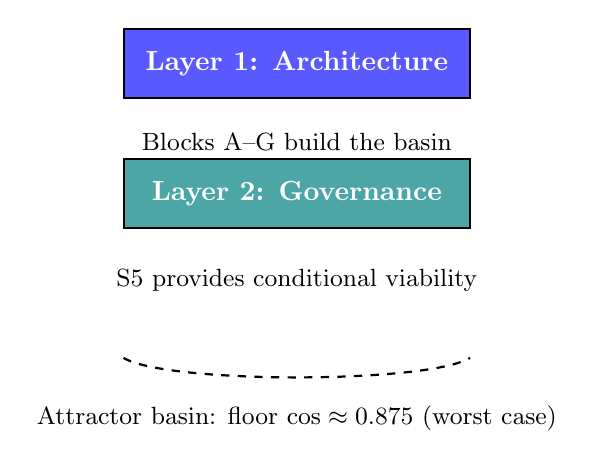
\begin{tikzpicture}[scale=1.1]
  \draw[thick, fill=blue!65] (0,3) rectangle (4,3.8);
  \node at (2,3.4) [text=white, font=\bfseries] {Layer 1: Architecture};
  \node at (2,2.5) {\small Blocks A--G build the basin};

  \draw[thick, fill=teal!70] (0,1.5) rectangle (4,2.3);
  \node at (2,1.9) [text=white, font=\bfseries] {Layer 2: Governance};
  \node at (2,0.9) {\small S5 provides conditional viability};

  \draw[dashed, thick] (0,0) .. controls (0.5,-0.3) and (3.5,-0.3) .. (4,0);
  \node at (2,-0.7) {\small Attractor basin: floor $\cos \approx 0{.}875$ (worst case)};
\end{tikzpicture}
\caption{Architecture builds the basin and its homeostasis; governance is the
difference between surviving stress and collapsing under it.}
\label{fig:two_layers}
\end{figure}

\begin{description}
  \item[\textbf{Layer 1: Architecture}] The arrangement of VSM blocks physically
        determines which regions of state space are habitable. The bare substrate
        (without blocks) drifts off-target and never stabilises; the blocks are what
        creates the point sink in $\R^{128}$.
  \item[\textbf{Layer 2: Governance (S5)}] At rest, governance is \emph{redundant}
        --- the system converges with or without it. Under stress it is decisive.
        Governance has two arms: a \emph{reactive} one (the algedonic safety response
        that regulates runaway thermal load) and a \emph{deliberative} one (the
        constitutional veto of the covenant, which can halt the system's own
        autonomy). The experiments exercise both.
\end{description}

With both layers present the system sustains viability at $\cos \approx 0{.}875$
(on a $0$--$1$ scale, with $0{.}70$ as the viability threshold) even under maximum
impulsive stress --- a margin of $0{.}175$ never breached in any experiment.

% ==============================================================================
\section*{The Closure: an Operationally Closed System}

The final experiment ran the complete kernel with all five Beer systems (S1--S5)
active under a single perturbation. Each level acted within its own cybernetic
scope. The decisive observation traverses the full model in a single tick: operations
(S1) registered a drop, coordination (S2) delivered a policy signal, control (S3)
detected the degradation and \emph{attempted} a correction, and policy (S5)
\emph{vetoed} it --- after which the system self-recovered. A separate test confirmed
the constitutional veto end-to-end: it halts autonomous control under sustained
degradation and restores it only on an explicit, cryptographically recorded human
resumption.

This is the sense of the architecture: not a simulation of Beer's diagram, but a
system in which every arrow carries a measured event.

% ==============================================================================
\section*{Empirical Results}

\begin{tabular}{lrl}
\textbf{Property} & \textbf{Measurement} & \textbf{Status} \\
\hline
Lyapunov exponent       & $\lambda_\text{max} = \ln(0{.}99) < 0$   & Measured, sink \\
Basin volume            & $\approx 1{.}0$ (reachable region)        & Monte-Carlo \\
Topology                & $\beta_0 = 1,\ \beta_1 = 0$               & No limit cycle \\
Basin uniqueness        & $\cos_\text{avg.\ paired} = 0{.}9854$     & Confirmed \\
Thermal viability       & viable at $68\,^\circ\mathrm{C}$          & Sustained \\
Basin floor             & $\cos \approx 0{.}875$                    & Margin $0{.}175$ \\
Entropy drop            & $\Delta H = 0{.}31$ bits                  & Constitutive \\
Viability certificate   & $V = \min(g,c,t,m),\ g = 0{.}102$        & Discriminates \\
Process governance      & 4 OS processes, $\tau = 1{.}0$            & cgroup~v2 live \\
VSM operational closure & S1--S5 causal in one run                  & Demonstrated \\
\hline
External coupling (S1)  & 12 zones, ERA5 live data                  & Operational \\
Markov projections (S4) & $P(\text{exc.}_{t+7d})$ per zone, NATS    & Operational \\
\end{tabular}

% ==============================================================================
\section*{What This Means}

\begin{enumerate}
  \item \textbf{Viability is geometric.} The system's stability emerges from the
        geometry of its state space, not from an external imposition. This is what
        Beer meant by a \emph{viable system}.

  \item \textbf{Ethical constraints enter as feasibility conditions.} The axioms
        prohibiting harm and coercion are not added on top --- a covenant violation
        collapses viability ($V \to 0$) exactly as exhausting the CPU budget does.
        The mathematics is \emph{indifferent} to what the constraints encode
        ethically; that indifference is precisely what makes it a general certifier
        rather than a moral theory.

  \item \textbf{Governance is conditional resilience.} A good policy layer does not
        \emph{create} viability --- architecture does --- but it is the difference
        between graceful survival and collapse when the system is challenged.

  \item \textbf{The basin is deep.} Under every perturbation tested the system never
        approached the viability threshold ($0{.}70$); the closest approach was
        $0{.}875$, a margin of $12{.}5\%$ above failure.

  \item \textbf{Anticipation requires environment.} A fully homeostatic system cannot
        anticipate itself: the regularity that stabilises it is the same regularity
        that flattens the anticipatory signal. External variance --- in this case,
        real climatic variability across twelve zones --- is a structural requirement
        of the S4 channel, not a design option.
\end{enumerate}

% ==============================================================================
\section*{Honest Limits}

The work runs on a single hardware node; the thermal stressor, although it raises the
actual silicon temperature, is a synthetic load; and the convergence experiments are
closed-system runs. The external coupling is operational, but the attractor's response
curve to sustained long-term signals is still work in progress: we have the
projections, but not yet a measure of how the kernel integrates them under real
climatic variability maintained over weeks or months.

The distributed architecture (eight LXC containers on a single Proxmox hypervisor)
is internal to the same system it measures: the resilience results hold under that
hardware profile, and extension to multiple nodes or heterogeneous workloads
(databases, inference) is future work.

% ==============================================================================
\section*{Next Steps}

\begin{enumerate}
  \item \textbf{Attractor response to sustained external environment.} With the
        climate network operational and the Markov projections online, the open
        question is how the attractor geometry responds to signals maintained over
        weeks: does the centroid shift? does the basin volume change? do excursions
        appear that the closed attractor does not produce?
  \item \textbf{Inter-system coordination via a formal substrate.} A parallel line
        of work studies whether two heterogeneous models can coordinate as distinct
        VSM layers through a shared formal language (VSL) --- the basis of a second
        paper.
  \item \textbf{\vOS{} on bare metal.} Deploying the kernel against real workloads
        (databases, inference) to measure attractor geometry under diverse load
        profiles and estimate the Landauer boundary of computational viability.
\end{enumerate}

% ==============================================================================
\section*{Acknowledgements}

The author thanks Marta Cinto, Ricardo Alfaro, Alejandra Rosales, and Marco Trigo
for making space to hear this work. Professor Ra\'{u}l Fierro (Universidad de
Valpara\'{i}so) generously reviewed an earlier draft; his observations improved the
presentation of the results.

% ==============================================================================
\section*{For the Beer Community}

This work returns to first principles: \emph{what does it mean for a system to be
viable?} We give a computational answer grounded in cybernetic axioms, using
instruments --- Benettin's algorithm, persistent homology, cryptographic attestation,
Markov chains over climatic history --- that did not exist when Beer wrote. The
architecture--governance distinction, and the demonstration that all five systems
close an operational loop on real hardware, suggest that the VSM blocks are not
metaphors: they are viability requirements with measurable geometry.

There are questions this work cannot answer on its own. Does the
architecture--governance distinction have a counterpart in real organisational
systems, or is it an artefact of the computational implementation? Is the threshold
$\cos \geq 0{.}70$ an invariant that makes sense for heterogeneous systems
(organisations, networks, institutions), or is it specific to this kernel? What does
someone who has worked with VSM in the field see when they read the ablation curve?

The full paper ($\approx$70 pages), data, and experimental logs are available on
request. So is the conversation.

\end{document}
